\documentclass[aspectratio=169]{beamer}
\usetheme{metropolis}

\usepackage[utf8]{inputenc}
\usepackage[T1]{fontenc}
\usepackage{graphicx}
\usepackage{booktabs}
\usepackage{fontawesome5} % for icons
\usepackage{pifont}       % for checkmarks
\usepackage{xcolor}       % for color definitions
\usepackage{colortbl}     % for \rowcolor, \rowcolors, \cellcolor in tables
\usepackage{tikz}         % for drawing graphics
\usetikzlibrary{patterns,positioning} % enable patterns and positioning for tikz
\usepackage{pgfplots}
\usepackage[transitions={dissolve}]{pdfpc}
%\pgfplotsset{compat=1.17} % set PGFPlots compatibility

% Colours
\definecolor{keystoneblue}{RGB}{0,77,128}
\definecolor{warmaccent}{RGB}{255,140,0}
\setbeamercolor{structure}{fg=keystoneblue}
\setbeamertemplate{navigation symbols}{}
\setbeamertemplate{footline}[frame number]

% Styling tweaks
\metroset{block=fill,progressbar=frametitle,numbering=fraction}
\renewcommand{\baselinestretch}{1.05}
\setbeamertemplate{frametitle}[default][center]

% Title and Author
\title[Evaluating RISC-V Enclaves]{\textbf{Evaluating RISC-V Enclaves:}\\ Security Without the Slowdown?}
\subtitle{Performance Evaluation and Optimization of Keystone Enclaves on RISC-V}
\author{\textbf{Basil Ugbomoiko}}
\institute[UzL]{Universität zu Lübeck \\ Institut für Technische Informatik}
\date{Master’s Thesis Defense — \today}
% Add logo (adjust path as needed)
\titlegraphic{\hfill\includegraphics[height=1.5cm]{uzl-logo.pdf}}
\begin{document}

% Title Page with University Logo (if available)
\begin{frame}
  \titlepage
  \vfill
  \centering\small\textit{In the age of untrusted infrastructure, can security keep up with performance?}
\end{frame}

% Opening Question Frame (Increased vertical space)
\begin{frame}{Opening Question}
\centering
\Huge\bfseries
Can we \textcolor{keystoneblue}{trust} computation on machines we \textcolor{warmaccent}{don't control}? \\[1em]
\large In cloud and edge scenarios, this question is no longer optional — it's urgent.
\end{frame}

\begin{frame}{Problem Statement: Trends}
\begin{itemize}
    \item[\faCloud] Growing reliance on \textcolor{warmaccent}{cloud} and \textcolor{warmaccent}{edge} computing.
    \item[\faUsers] Shared, multi-tenant infrastructure is the norm.
\end{itemize}
\end{frame}

\begin{frame}{Problem Statement: Challenge}
\begin{itemize}
    \item[\faExclamationTriangle] Traditional security assumes a trustworthy OS — \alert{assumption broken}.
    \item[\faLock] Need isolation of critical code/data \textbf{even if the OS is compromised}.
\end{itemize}
\vfill
%\scriptsize\textit{This sets the stage for Trusted Execution Environments (TEEs).}
\begin{figure}[h]
\centering
\begin{tikzpicture}[node distance=1.2cm and 1cm, every node/.style={font=\small}]
    \node[draw, fill=orange!30, minimum width=2.5cm, minimum height=1cm, rounded corners] (app) {\textbf{App}};
    \node[draw, fill=gray!20, below=of app, minimum width=3cm, minimum height=1cm, rounded corners] (os) {\textbf{Untrusted OS}};
    \node[draw, fill=blue!15, right=3cm of app, minimum width=2.5cm, minimum height=1cm, rounded corners] (enclave) {\faLock\ \textbf{Enclave}};
    
    \draw[->, thick, red] (os) -- (app) node[midway, left, align=left, font=\footnotesize] {Possible interference\\ or data snooping};
    \draw[->, thick, keystoneblue] (app) -- (enclave) node[midway, above, font=\footnotesize] {Trusted Execution};
    \draw[->, thick, dashed, red] (os) -- (enclave) node[midway, below, font=\footnotesize] {Attempted attack blocked};
\end{tikzpicture}
\caption{Enclaves isolate computation from a compromised OS}
\end{figure}
\end{frame}

% Research Gap (Emphasized visual structure)
\begin{frame}{Research Gap}
\centering
\Large\bfseries
No comprehensive, benchmarked assessment of \\
\textbf{Keystone} performance overhead with \\
\textit{actionable tuning guidance.}
\end{frame}

\begin{frame}{Contributions}
\begin{itemize}
    \item \textbf{Systematic performance evaluation} of Keystone across varied workloads.
    \item \textbf{Identification of hardware bottlenecks} like PMP entry exhaustion and misaligned memory.
    \item \textbf{Actionable optimization guidelines} for developers using Keystone TEEs.
    %\item \textbf{Visual benchmarking workflow} and comparison to alternative TEEs.
\end{itemize}
\end{frame}

\section{Background and System Design}

% Background on TEEs (Added icons for clarity)
\begin{frame}{Background: TEEs in a Nutshell}
\begin{block}{Definition}
Hardware-based secure “zones” for executing sensitive code and storing sensitive data.
\end{block}
Examples include:
\begin{itemize}
    \item Intel SGX \faMicrochip\ \textit{(Intel's enclave solution for secure execution)} 
    \item ARM TrustZone \faLock\ \textit{(Security for mobile devices)}
    \item AMD SEV \faServer\ \textit{(Virtual machine encryption for server environments)}
    \item Keystone \faKey\ \textit{(Modular, open-source for RISC-V)}
\end{itemize}
\end{frame}

% % Research Objectives (Visual appeal with bullet style)
% \begin{frame}{Research Objectives}
% \begin{enumerate}
%     \item Characterize Keystone’s \textbf{architecture} and \textbf{security model}.
%     \item Quantify performance across \textcolor{warmaccent}{varied workloads}.
%     \item Recommend \textbf{best practices} for optimal configuration.
% \end{enumerate}
% \end{frame}

% What is RISC-V? Slide
\begin{frame}{What is RISC-V?}
\begin{itemize}
    \item Open-source, modular processor architecture.
    \item Highly customizable for specialized hardware (ideal for enclaves).
    \item Scalable from embedded systems to high-performance computing.
    \item Growing adoption in academia and industry (e.g., SiFive, Western Digital).
\end{itemize}
\begin{block}{Key Concept}
\textit{RISC-V’s open-source nature enables flexible, secure processor designs for enclave-based systems.}
\end{block}
\end{frame}

% Keystone 
\begin{frame}{From Problem to Solution: Enter Keystone}
    \only<1>{
\begin{block}{What is Keystone?}
\begin{itemize}
    \item Modular, open-source TEE for RISC-V.
    \item Uses Physical Memory Protection (PMP) and minimal Security Monitor for isolation.
    \item Low Trusted Computing Base (TCB) for security and flexibility.
    %\item Optimized for secure computation in untrusted environments.
\end{itemize}
\end{block}
    }
% \begin{block}{Key Concept}
% \textit{Low TCB reduces attack surfaces while enabling high flexibility and performance in enclave-based systems.}
% \end{block}
%\end{frame}

% Keystone Framework Architecture
%\begin{frame}{Keystone Framework Architecture}
%     \only<1>{
% \begin{block}{Overview}
%     Keystone is designed to be modular, with clear isolation between enclaves and the OS.
% \end{block}
%     }
%     \only<2>{
%\resizebox{\linewidth}{!}{%
\only<2>{
\begin{figure}[htbp]
\centering
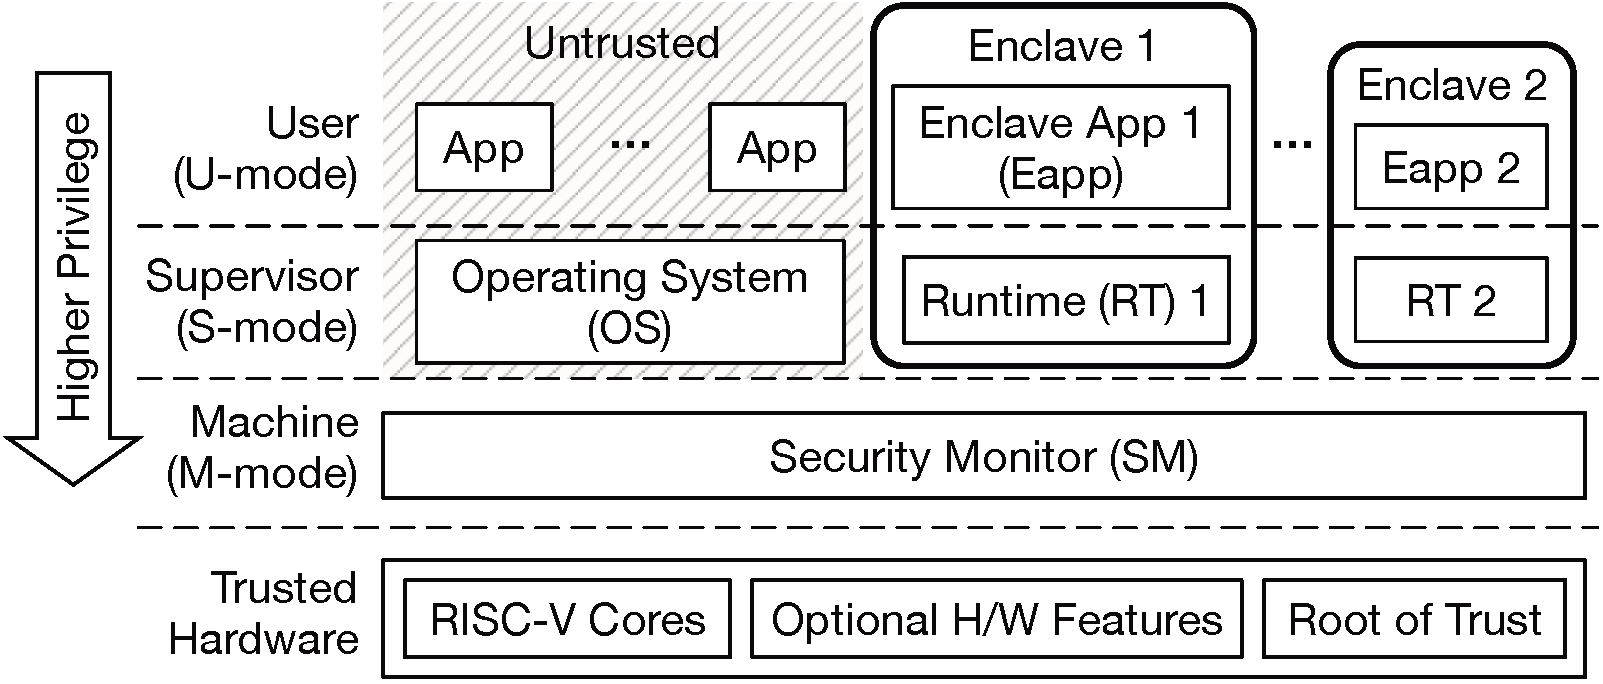
\includegraphics[width=\linewidth]{/home/individual-01/Documents/keystone-thesis/figures/keystone_overview.png}
\caption{Keystone architecture showing components such as the Security Monitor, enclave runtime, and the privilege hierarchy.}
\label{fig:keystone_grouped}
\end{figure}
    }
%\end{frame}

% Keystone vs Other TEEs
%\begin{frame}{Keystone vs. Other TEEs}
\only<3>{
\begin{figure}[htbp]
\centering
\renewcommand{\arraystretch}{1.3} % more row height
\setlength{\tabcolsep}{5pt}       % more column padding
\rowcolors{2}{gray!5}{white}      % alternating row colors

\begin{tabular}{@{}lcccc@{}}
\toprule
\rowcolor{gray!20}
\textbf{Feature} & \textbf{Keystone} & \textbf{SGX} & \textbf{TrustZone} & \textbf{SEV} \\
\midrule
Open Source            & \cellcolor{green!15}Yes & \cellcolor{red!15}No & \cellcolor{red!15}No & \cellcolor{red!15}No \\
Dynamic Enclaves       & \cellcolor{green!15}Yes & \cellcolor{red!15}No & \cellcolor{yellow!15}Limited & \cellcolor{red!15}No \\
Hardware Dependency    & \cellcolor{green!15}RISC-V & \cellcolor{red!15}Intel & \cellcolor{red!15}ARM & \cellcolor{red!15}AMD \\
TCB Size               & \cellcolor{green!15}Low & \cellcolor{yellow!15}Medium & \cellcolor{red!15}High & \cellcolor{yellow!15}Medium \\
Flexible Configurations& \cellcolor{green!15}High & \cellcolor{red!15}Low & \cellcolor{red!15}Low & \cellcolor{yellow!15}Medium \\
\bottomrule
\end{tabular}
\caption{Feature comparison of major TEEs.}
\label{fig:tee-features}
\end{figure}
}
\end{frame}

\section{Experimental Setup}

\begin{frame}{System Design and Methodology}
    \small
    \begin{itemize}
        \item \textbf{Objective:} Evaluate the performance impact of Keystone's enclave isolation mechanisms on embedded/system-level workloads. \pause
        \item \textbf{Platform:} Emulated RISC-V architecture (RV64GC) using QEMU. \pause
        \item \textbf{Focus:} Quantify computational overhead when using Keystone enclaves vs. traditional non-isolated execution. \pause
    \end{itemize}
    \vspace{0.5em}
    \uncover<4->{\textbf{Platform Configuration: QEMU-based emulation ensures controlled environment for testing.}}
\end{frame}

% \begin{frame}{QEMU-Based Virtualized Environment}
%     \small
%     \begin{itemize}
%         \item QEMU emulates RISC-V architecture for repeatability and control. \pause
%         \item Ensures consistent test conditions by eliminating hardware-induced variations (thermal throttling, cache behavior). \pause
%         \item Configured for RV64GC architecture, as required by Keystone. \pause
%     \end{itemize}
%     \vspace{0.5em}
%     \uncover<4->{\textbf{Why QEMU?} Provides a controlled, consistent environment for repeatability.}
% \end{frame}

\begin{frame}{Benchmarking Workflow}
    \small
    \begin{itemize}
        \item \textbf{Define benchmark set} and configure system setup. \pause
        \item \textbf{Dual-mode execution:} Run benchmarks in native mode (without enclave) and enclave mode (with isolation). \pause
        \item \textbf{Metrics collection:} Gather data on execution time, throughput, and overhead. \pause
        \item \textbf{Analysis:} Compare performance across modes and assess overheads. \pause
    \end{itemize}
    \vspace{0.5em}
    %\uncover<5->{\textbf{Visual Workflow:} As shown in Figure \ref{fig:benchmarking-swimlane}, the process starts with benchmarking selection and proceeds through dual-mode execution.}
    \begin{figure}[H]
    \centering
\begin{figure}[htbp]
\centering
\resizebox{\linewidth}{!}{%
\begin{tikzpicture}[
    >=stealth,
    phase/.style={
        font=\bfseries\small,
        text=white,
        minimum height=0.8cm,
        rounded corners,
        inner xsep=6pt,
        text centered
    },
    stepnode/.style={
        draw=black!70,
        thick,
        rounded corners,
        align=center,
        font=\scriptsize,
        minimum height=1.4cm,
        text width=2.8cm,
        inner sep=6pt
    },
    arrow/.style={->, thick, shorten >=2pt, shorten <=2pt}
]

% Top row (Setup & Config) - blue shades
\node[stepnode, fill=blue!15] (s1) at (0,3) {\faTasks\\Define benchmarks};
\node[stepnode, fill=blue!20, right=1.8cm of s1] (s2) {\faMicrochip\\Select hardware};

% Bottom row (Execution & Analysis) - green shades
\node[stepnode, fill=green!15, right=1.8cm of s2] (s3) {\faPlay\\Run native mode};
\node[stepnode, fill=green!20, right=1.8cm of s3] (s4) {\faLock\\Run enclave mode};
\node[stepnode, fill=green!25] (s5) at (0,1) {\faChartBar\\Collect metrics};
\node[stepnode, fill=green!30, right=1.8cm of s5] (s6) {\faSearch\\Analyze overheads};
\node[stepnode, fill=green!40, right=1.8cm of s6] (s7) {\faArchive\\Archive results};

% Arrows top row
\draw[arrow] (s1) -- (s2);
\draw[arrow] (s2) -- (s3);
\draw[arrow] (s3) -- (s4);

% Arrow from top to bottom
\draw[arrow] (s4.south) .. controls +(0,-0.8) and +(0,0.8) .. (s5.north);

% Arrows bottom row
\draw[arrow] (s5) -- (s6);
\draw[arrow] (s6) -- (s7);

% Color legend
\node[draw=black!50, fill=white, rounded corners, align=left, font=\scriptsize, anchor=north west] 
    at ([xshift=1cm,yshift=-0.5cm]s7.south east) (legend) {
    \begin{tikzpicture}[baseline=(current bounding box.center)]
        \node[fill=blue!20, minimum width=0.5cm, minimum height=0.5cm] (b) {};
        \node[right=0.3cm of b, anchor=west] {Setup \& Config};
        \node[fill=green!30, minimum width=0.5cm, minimum height=0.5cm, below=0.2cm of b] (g) {};
        \node[right=0.3cm of g, anchor=west] {Execution \& Analysis};
    \end{tikzpicture}
};

\end{tikzpicture}
}
\caption{Benchmarking and data collection workflow}
\end{figure}
    \caption{Benchmarking and data collection workflow}
    \label{fig:benchmarking-swimlane}
    \end{figure}
\end{frame}

% \begin{frame}{Benchmarking Tools}
%     \small
%     \begin{itemize}
%         \item \textbf{Dhrystone:} Measures CPU performance (DMIPS).
%         \item \textbf{CoreMark:} Focuses on integer performance, used in embedded systems benchmarking.
%         \begin{block}{Execution Modes}
%         \begin{itemize}
%             \item \textbf{Native Execution:} Benchmark runs as a normal process.
%             \item \textbf{Enclave Execution:} Benchmark runs within a Keystone enclave.
%         \end{itemize}
%         \end{block}
%     \end{itemize}
%     %\vspace{0.5em}
%     %\uncover<1->{\textbf{Key Focus:} These tools provide insights into both CPU-bound and system-level performance.}
% \end{frame}

%Results
\section{Results and Hardware Bottlenecks}
\label{sec:synthesis}

\begin{frame}{Enclave Overhead and System Behavior}
\small
% First overlay: text only
\only<1>{
\begin{block}{Performance Overhead}
\begin{itemize}
    \item \textbf{Enclave execution} introduces overhead:
        \begin{itemize}
            \item Compute-bound workloads like CoreMark and Dhrystone incur moderate overhead of 1.06$\times$ to 1.61$\times$.
            \item Hybrid workloads (Compute- and memory-bound) like Kyber suffer severe overhead, up to 2.73$\times$.
        \end{itemize}
    %\item \textbf{Memory-bound workloads} experience significant penalties due to enclave-induced memory isolation and security checks.
\end{itemize}
\end{block}
}

\only<2>{
% \begin{frame}{Performance Trends and Hardware Bottlenecks}
\centering
\begin{figure}[htbp]
\centering
\begin{tikzpicture}
\begin{axis}[
    ybar,
    bar width=14pt,
    width=10cm,
    height=6cm,
    ymin=0, ymax=120,
    ylabel={Relative performance (\%)},
    symbolic x coords={CoreMark,Dhrystone,Kyber},
    xtick=data,
    ymajorgrids,
    grid style=dashed,
    nodes near coords,
    every node near coord/.append style={font=\footnotesize, /pgf/number format/fixed},
    legend style={at={(0.5,-0.15)}, anchor=north, legend columns=-1}
]

% Native: orange, rounded top, tranRecommendationssparency
\addplot[
    fill={rgb,255:red,230; green,159; blue,0},
    fill opacity=0.8,
    draw=black!60,
    rounded corners=2pt
] coordinates {(CoreMark,100) (Dhrystone,100) (Kyber,100)};

% Enclave: blue, rounded top, transparency
\addplot[
    fill={rgb,255:red,0; green,114; blue,178},
    fill opacity=0.8,
    draw=black!60,
    rounded corners=2pt
] coordinates {(CoreMark,95) (Dhrystone,62) (Kyber,37)};

\legend{Native,Enclave}
\end{axis}
\end{tikzpicture}
\caption{Relative performance of enclave vs native execution.}
\end{figure}
}
\end{frame}

% % Second overlay: add figure
% \only<3>{
% \begin{block}{Overhead Breakdown}
% \begin{itemize}
%     \item Memory isolation via PMP adds fixed latency per memory access.
%     \item Context switches between host and enclave domains are costly.
% \end{itemize}
% \end{block}
% }
% \centering
% \textbf{Key Insight:} Overhead varies based on workload characteristics and memory behavior.
% \end{frame}
% Figure appears only on the second slide of this frame

\begin{frame}{Impact of Scalability Limitations}
\small
\only<1>{
\begin{block}{CPU Scaling Limits}
\begin{itemize}
    \item Increasing CPU cores \textbf{benefits multi-threaded tasks}, but gains plateau due to context-switch overhead.
    \item For example, \texttt{CoreMark} shows marginal improvements beyond 4 cores.
\end{itemize}
\end{block}
\centering
\begin{tikzpicture}
\begin{axis}[
    ybar,
    bar width=8pt,
    width=0.75\linewidth,
    height=4.2cm,
    enlarge x limits=0.15,
    ymin=95, ymax=125,
    xlabel={CPU cores},
    ylabel={Rel.\ perf.\ (\%)},
    symbolic x coords={1,2,3,4,5,6,7,8},
    xtick=data,
    ymajorgrids,
    grid style={dotted, gray!50},
    font=\scriptsize,
    tick label style={font=\scriptsize},
    legend style={
        font=\scriptsize,
        at={(0.5,-0.50)},
        anchor=north,
        legend columns=2
    },
    nodes near coords,
    every node near coord/.append style={font=\tiny},
    point meta=explicit symbolic
]

% Native
\addplot[fill=blue!40] coordinates {
    (1,100) [100]
    (2,108) [108]
    (3,115) [115]
    (4,120) [120]
    (5,122) [122]
    (6,123) [123]
    (7,123) [123]
    (8,123) [123]
};

% Enclave
\addplot[fill=green!50!black!40] coordinates {
    (1,100) [100]
    (2,102) [102]
    (3,103) [103]
    (4,104) [104]
    (5,106) [106]
    (6,108) [108]
    (7,110) [110]
    (8,110) [110]
};

\legend{Native, Enclave}
\end{axis}
\end{tikzpicture}


}
\only<2>{
\begin{block}{Memory Scaling Constraints}
\begin{itemize}
    \item Increased memory capacity \textbf{improves performance} by reducing page faults.
    \item \textbf{Fragmentation} and \textbf{PMP entry limits} cap the performance improvement.
\end{itemize}
\end{block}
\centering
\begin{tikzpicture}
\begin{axis}[
    ybar,
    bar width=8pt,
    width=0.75\linewidth,
    height=4.2cm,
    enlarge x limits=0.2,
    ymin=90, ymax=118,
    xlabel={Memory (MB)},
    ylabel={Rel.\ perf.\ (\%)},
    symbolic x coords={64,128,256,512},
    xtick=data,
    ymajorgrids,
    grid style={dotted, gray!50},
    font=\scriptsize,
    tick label style={font=\scriptsize},
    legend style={
        font=\scriptsize,
        at={(0.5,-0.5)},
        anchor=north,
        legend columns=1
    },
    nodes near coords,
    every node near coord/.append style={font=\tiny},
    point meta=explicit symbolic
]

% Native contiguous
\addplot[fill=blue!40] coordinates {
    (64,100) [100]
    (128,106) [106]
    (256,112) [112]
    (512,115) [115]
};

% Enclave contiguous
\addplot[fill=green!50!black!40] coordinates {
    (64,95) [95]
    (128,98) [98]
    (256,100) [100]
    (512,102) [102]
};

% Enclave fragmented
\addplot[fill=orange!70!black!40] coordinates {
    (64,92) [92]
    (128,94) [94]
    (256,95) [95]
    (512,96) [96]
};

\legend{Native contig., Enclave contig., Enclave frag.}
\end{axis}
\end{tikzpicture}

}
% \centering
% \textbf{Key Insight:} Hardware resources alone cannot fully predict enclave performance due to system resource allocation limits.
\end{frame}

\begin{frame}{PMP Entry Exhaustion and Multi-Enclave Scalability}
\small
\only<1>{
\begin{block}{PMP Resource Limitations}
\begin{itemize}
    \item \textbf{Maximum PMP entries}: 16.
    \item Exhausted PMP entries \textbf{prevent new enclave creation}, causing errors even with abundant system resources.
    \item Failure due to PMP exhaustion: \texttt{SBI error codes}.
\end{itemize}
\end{block}
}
\only<2>{
\begin{block}{Scalability Bottleneck}
\begin{itemize}
    \item In \textbf{multi-tenant environments}, PMP exhaustion limits the number of concurrent enclaves.
    \item This creates scalability issues, especially for high-concurrency workloads.
\end{itemize}
\end{block}
}

% \centering
% \textbf{Key Insight:} PMP limitations represent a significant scalability bottleneck for RISC-V enclave-based systems.
% \end{frame}


% \begin{frame}{Key Takeaways from Performance Trends}
% \small
% \begin{block}{Main Findings}
% \begin{itemize}
%     \item Enclave performance suffers primarily in \textbf{memory-bound workloads} due to security checks and context switching.
%     \item \textbf{PMP entry limitations} restrict scalability in multi-enclave setups.
%     \item Increasing hardware resources does not linearly translate to performance gains due to system-level overheads.
% \end{itemize}
% \end{block}

% \centering
% \textbf{Key Insight:} Optimizing both hardware resources and system-level configurations is essential for scalable and efficient enclave execution.
% \end{frame}


% \begin{frame}{Why Misalignment Bloats PMP Usage}
% \small
% \vfill

% % Problem
% \only<1>{
% \begin{block}{Problem}
% Physical Memory Protection (PMP) entries must cover power‑of‑two sized, naturally aligned regions (NAPOT).
% \end{block}
% }

% % Cause
% \only<2>{
% \begin{block}{Problem}
% Physical Memory Protection (PMP) entries must cover power‑of‑two sized, naturally aligned regions (NAPOT).
% \end{block}
% \vspace{0.5em}
% \begin{block}{Cause}
% When a memory region is \textbf{misaligned}:
% \begin{itemize}
%   \item NAPOT encoding forces padding to the next power‑of‑two boundary.
%   \item Padding areas consume PMP coverage even if they are not actual data.
% \end{itemize}
% \end{block}
% % \draw[->, thick] (0,-0.2) -- (0,-0.8); % optional arrow from Problem → Cause
% }

% % Effect
% \only<3>{
% \begin{block}{Cause}
% When a memory region is \textbf{misaligned}:
% \begin{itemize}
%   \item NAPOT encoding forces padding to the next power‑of‑two boundary.
%   \item Padding areas consume PMP coverage even if they are not actual data.
% \end{itemize}
% \end{block}
% \vspace{0.5em}
% \begin{block}{Effect}
% \begin{itemize}
%   \item A single logical region may require \textbf{multiple PMP entries}.
%   \item Fragmentation increases as more regions are misaligned.
% \end{itemize}
% \end{block}
% % \draw[->, thick] (0,-0.2) -- (0,-0.8); % optional arrow from Cause → Effect
% }

% % Impact
% \only<4>{
% \begin{block}{Effect}
% \begin{itemize}
%   \item A single logical region may require \textbf{multiple PMP entries}.
%   \item Fragmentation increases as more regions are misaligned.
% \end{itemize}
% \end{block}
% \vspace{0.5em}
% \begin{block}{Impact}
% \begin{itemize}
%   \item Higher PMP entry count $\Rightarrow$ fewer entries left for other regions.
%   \item Limits scalability and flexibility of memory protection.
%   \item Wastes address space and complicates security policy.
% \end{itemize}
% \end{block}
% }

% % Key takeaway
% \only<5>{
% \centering
% \begin{figure}[htbp]
% \centering
% \begin{tikzpicture}[scale=1, transform shape,font=\small]

% % Memory axis
% \draw[thick,->] (0,0) -- (10,0) node[anchor=west]{Memory address};
% \foreach \x/\label in {0/0\,KB,1.25/128\,KB,4.25/192\,KB,8/300\,KB}
%     \draw (\x,0.1) -- (\x,-0.1) node[anchor=north]{\label};

% % === Region 1: contiguous, 1 PMP entry ===
% \node[anchor=south] at (1.375,2.1) {\scriptsize 128\,KB aligned};
% %\draw[pattern=north east lines,pattern color=black] (0.25,0) rectangle (0.5,1);
% \draw[fill=keystoneblue!60] (0.5,0) rectangle (2.2,1);
% %\draw[pattern=north east lines,pattern color=black] (2.2,0) rectangle (2.5,1);
% \draw[fill=keystoneblue!60,opacity=0.4] (0.5,1) rectangle (2.2,2) node[pos=.5] {\scriptsize 1 entry};

% % === Region 2: fragmented, 3 PMP entries ===
% \node[anchor=south] at (4.3,4.1) {\scriptsize 192\,KB misaligned};
% \draw[pattern=north east lines,pattern color=black] (3.5,0) rectangle (3.8,1);
% \draw[fill=warmaccent!60] (3.8,0) rectangle (4.6,1);
% \draw[pattern=north east lines,pattern color=black] (4.6,0) rectangle (5.1,1);
% \draw[fill=warmaccent!60,opacity=0.4] (3.5,1) rectangle (5.1,4) node[pos=.5] {\scriptsize 3 entries};

% % === Region 3: fragmented, 3 PMP entries ===
% \node[anchor=south] at (8.0,4.1) {\scriptsize 300\,KB misaligned};
% \draw[pattern=north east lines,pattern color=black] (6.7,0) rectangle (7.0,1);
% \draw[fill=warmaccent!60] (7.0,0) rectangle (9.1,1);
% \draw[pattern=north east lines,pattern color=black] (9.1,0) rectangle (9.3,1);
% \draw[fill=warmaccent!60,opacity=0.4] (6.7,1) rectangle (9.3,4) node[pos=.5] {\scriptsize 3 entries};

% % Arrows showing cause-effect
% %\draw[->,thick] (2.2,0.5) .. controls (2.8,1.5) .. (3.4,2) node[midway,above,sloped]{\scriptsize Padding $\Rightarrow$ More entries};
% \draw[->,thick] (5.1,0.5) .. controls (5.4,2) .. (6.6,2.5) node[midway,above,sloped]{\scriptsize Padding $\Rightarrow$ More entries};

% % Legend
% \begin{scope}[xshift=0cm,yshift=-1.5cm]
% \draw[fill=keystoneblue!60] (0,0) rectangle (0.4,0.4) node[right=0.5cm] {Contiguous region};
% \draw[fill=warmaccent!60] (5,0) rectangle (5.4,0.4) node[right=0.5cm] {Fragmented region};
% \draw[pattern=north east lines,pattern color=black] (0,-0.6) rectangle (0.4,-0.2) node[right=0.5cm] {Wasted padding};
% \draw[fill=gray!50,opacity=0.4] (5,-0.6) rectangle (5.4,-0.2) node[right=0.5cm] {PMP entry count bar};
% \end{scope}

% \end{tikzpicture}

% \vspace{0.4em}
% \scriptsize
% \textbf{Takeaway:} Align regions to NAPOT boundaries to minimize padding and preserve PMP entries.
% \end{figure}
% }

% \vfill
% \end{frame}

% \begin{frame}{PMP Entries vs Max Concurrent Enclaves}
% \centering
\only<3>{
\begin{figure}[htbp]
\centering
\begin{tikzpicture}
\begin{axis}[
    width=10cm,
    height=6cm,
    xlabel={PMP Entries},
    ylabel={Concurrent Enclaves},
    xmin=0, xmax=16,
    ymin=0, ymax=16,
    xtick={0,4,8,12,16},
    ymajorgrids,
    grid style=dashed,
    mark options={solid},
    nodes near coords,
    every node near coord/.append style={font=\footnotesize, /pgf/number format/fixed},
    clip=false,
    cycle list={{teal,mark=*,thick}},
    tick label style={font=\small},
    label style={font=\small\bfseries},
]

% Data plot
\addplot[
    color=teal,
    mark=*,
    thick
] coordinates {
    (0,0) (2,2) (4,4) (6,6) (8,8) (10,8) (12,8) (14,8) (16,8)
};

% Highlight PMP exhaustion area
\fill[red!30,opacity=0.4] (axis cs:8,0) rectangle (axis cs:16,16);

% Add Yellow Sliding Zone (between 4 and 8 PMP entries)
\fill[yellow!30, opacity=0.6] (axis cs:4,0) rectangle (axis cs:8,16);

% Annotation inside shaded region
\node[red, align=center, font=\footnotesize\bfseries] at (axis cs:12,12) {PMP Exhaustion \\ Caps at 8 Enclaves};
\node[align=center, font=\footnotesize\bfseries, text=black] at (axis cs:6,12) {Sliding Zone};

% Stability boundary line & label
\draw[dashed, thick, color=blue] (axis cs:4,0) -- (axis cs:4,16);
\node[anchor=south, font=\footnotesize\bfseries, color=blue] at (axis cs:4,16) {Stability Boundary};

\end{axis}
\end{tikzpicture}
\caption{Max enclaves increase with PMP entries until exhaustion caps growth.}
\end{figure}
}
\end{frame}

\begin{frame}{PMP Misalignment: Why It Matters}
    \only<1>{
\begin{block}{The Problem}
PMP entries must describe power-of-two, naturally aligned regions (NAPOT). Misaligned memory allocations cause unnecessary padding.
\end{block}
    }
%     \only<2>{
% \begin{block}{The Effect}
% \begin{itemize}
%     \item Misalignment causes a single memory region to consume multiple PMP entries.
%     \item Fragmentation leads to rapid exhaustion of PMP resources (max = 16 entries).
% \end{itemize}
% \end{block}

% \vspace{1em}
% \centering
% \textbf{Next: Visualizing the impact →}
%\end{frame}
%     }
    \only<2>{
%\begin{frame}{PMP Misalignment: Visualized}
%\centering
\begin{figure}[htbp]
\centering
\begin{tikzpicture}[scale=1, transform shape,font=\small]

% Memory axis
\draw[thick,->] (0,0) -- (10,0) node[anchor=west]{Memory address};
\foreach \x/\label in {0/0\,KB,1.25/128\,KB,4.25/192\,KB,8/300\,KB}
    \draw (\x,0.1) -- (\x,-0.1) node[anchor=north]{\label};

% === Region 1: contiguous, 1 PMP entry ===
\node[anchor=south] at (1.375,2.1) {\scriptsize 128\,KB aligned};
\draw[fill=keystoneblue!60] (0.5,0) rectangle (2.2,1);
\draw[fill=keystoneblue!60,opacity=0.4] (0.5,1) rectangle (2.2,2) node[pos=.5] {\scriptsize 1 entry};

% === Region 2: fragmented, 3 PMP entries ===
\node[anchor=south] at (4.3,4.1) {\scriptsize 192\,KB misaligned};
\draw[pattern=north east lines,pattern color=black] (3.5,0) rectangle (3.8,1);
\draw[fill=warmaccent!60] (3.8,0) rectangle (4.6,1);
\draw[pattern=north east lines,pattern color=black] (4.6,0) rectangle (5.1,1);
\draw[fill=warmaccent!60,opacity=0.4] (3.5,1) rectangle (5.1,4) node[pos=.5] {\scriptsize 3 entries};

% === Region 3: fragmented, 3 PMP entries ===
\node[anchor=south] at (8.0,4.1) {\scriptsize 300\,KB misaligned};
\draw[pattern=north east lines,pattern color=black] (6.7,0) rectangle (7.0,1);
\draw[fill=warmaccent!60] (7.0,0) rectangle (9.1,1);
\draw[pattern=north east lines,pattern color=black] (9.1,0) rectangle (9.3,1);
\draw[fill=warmaccent!60,opacity=0.4] (6.7,1) rectangle (9.3,4) node[pos=.5] {\scriptsize 3 entries};

% Arrows showing cause-effect
\draw[->,thick] (5.1,0.5) .. controls (5.4,2) .. (6.6,2.5) node[midway,above,sloped]{\scriptsize Padding $\Rightarrow$ More entries};

% Legend
\begin{scope}[xshift=0cm,yshift=-1.5cm]
\draw[fill=keystoneblue!60] (0,0) rectangle (0.4,0.4) node[right=0.5cm] {Contiguous region};
\draw[fill=warmaccent!60] (5,0) rectangle (5.4,0.4) node[right=0.5cm] {Fragmented region};
\draw[pattern=north east lines,pattern color=black] (0,-0.6) rectangle (0.4,-0.2) node[right=0.5cm] {Wasted padding};
\draw[fill=gray!50,opacity=0.4] (5,-0.6) rectangle (5.4,-0.2) node[right=0.5cm] {PMP entry count bar};
\end{scope}

\end{tikzpicture}

\vspace{0.4em}
\scriptsize
\textbf{Takeaway:} Align regions to NAPOT boundaries to minimize padding and preserve PMP entries.
\end{figure}
    }
\end{frame}

% Optimizations for Keystone Enclaves
% \begin{frame}{Optimizations for Keystone Enclaves}
% \begin{itemize}
%     \item Use contiguous, NAPOT-aligned memory to minimize PMP usage.
%     \item Consolidate workloads and limit active enclaves to reduce contention.
%     \item Offload non-sensitive tasks to the untrusted domain.
% \end{itemize}
% \end{frame}

\section{Practical Deployment Strategies and Recommendations}

\begin{frame}{Deployment Takeaways}
\begin{block}{Best Practices}
\begin{itemize}
    \only<1>{\item \faMemory\ \textbf{Align memory precisely:} Use NAPOT-aligned, contiguous regions to simplify PMP configuration.}
    \only<2>{\item \faProjectDiagram\ \textbf{Minimize enclave count:} Consolidate workloads to reduce PMP entry usage and management overhead.
    \begin{tikzpicture}[font=\scriptsize,>=stealth]

% --- BEFORE: Multiple enclaves ---
\node[anchor=west] at (-0.5,2.5) {\textbf{Before: Multiple Enclaves}};
\foreach \i in {0,2.5,5} {
  % Enclave box
  \draw[fill=red!20,thick] (\i,1) rectangle +(2,1);
  \node at (\i+1,2.15) {Enclave};
  % Task inside
  \draw[fill=blue!10,thick] (\i+0.5,1.2) rectangle +(1,0.6);
  \node at (\i+1,1.5) {Task};
}

% Arrow between before and after (shorter gap)
\draw[->,thick] (3.5,0.8) -- (3.5,0.2) node[midway,right]{\textbf{Merge}};

% --- AFTER: Single consolidated enclave (moved up) ---
\node[anchor=west] at (-0.5,-0.6) {\textbf{After: Single Enclave}};
\draw[fill=green!20,thick] (0,-1.8) rectangle (7,-0.8);
\node at (3.5,-2.05) {Single Consolidated Enclave};

% Tasks inside consolidated enclave
\foreach \i in {0.5,3,5.5} {
  \draw[fill=blue!10,thick] (\i,-1.6) rectangle +(1,0.6);
  \node at (\i+0.5,-1.3) {Task};
}

% Optional legend
\begin{scope}[shift={(8,0)}]
  \draw[fill=red!20] (0,1.5) rectangle +(0.5,0.3);
  \node[right] at (0.6,1.65) {Separate Enclave};
  \draw[fill=green!20] (0,1) rectangle +(0.5,0.3);
  \node[right] at (0.6,1.15) {Consolidated Enclave};
  \draw[fill=blue!10] (0,0.5) rectangle +(0.5,0.3);
  \node[right] at (0.6,0.65) {Task};
\end{scope}


\end{tikzpicture}

    }
    \only<3>{\item \faRetweet\ \textbf{Reduce switching costs:} Batch enclave calls to limit context switches and improve throughput.
    \begin{figure}[H]
\centering
\begin{tikzpicture}[>=stealth,thick,font=\scriptsize,scale=0.9]
  % === Left: Unbatched ===
  \fill[green!10] (0,0) rectangle (2.5,2.5);
  \fill[blue!10] (2.5,0) rectangle (5,2.5);

  \node at (1.25,2.7) {\textbf{Enclave}};
  \node at (3.75,2.7) {\textbf{Host}};

  \draw[dashed,thick] (2.5,0) -- (2.5,2.5) node[midway,above,sloped];

  \draw[->,red!70!black] (0.8,2.0) -- (3.2,2.0) node[midway,above]{Call 1};
  \draw[->,red!70!black] (0.8,1.4) -- (3.2,1.4) node[midway,above]{Call 2};
  \draw[->,red!70!black] (0.8,0.8) -- (3.2,0.8) node[midway,above]{Call 3};

  \node[align=center] at (2.5,-0.6) {\textbf{Unbatched}\\Multiple crossings};

  % === Right: Batched ===
  \begin{scope}[shift={(6,0)}]
    \fill[green!10] (0,0) rectangle (2.5,2.5);
    \fill[blue!10] (2.5,0) rectangle (5,2.5);

    \node at (1.25,2.7) {\textbf{Enclave}};
    \node at (3.75,2.7) {\textbf{Host}};

    \draw[dashed,thick] (2.5,0) -- (2.5,2.5) node[midway,above,sloped];

\draw[->,red!70!black,thick] (0.8,1.3) -- (2.8,1.3) 
    node[midway,above]{Batched Call}
    node[midway,below=4pt,draw,fill=orange!20,rounded corners=2pt,
         inner xsep=4pt,inner ysep=2pt]{Batch Processor};

    \node[align=center] at (2.5,-0.6) {\textbf{Batched}\\One crossing};
  \end{scope}

\end{tikzpicture}
%\caption{Unbatched vs Batched enclave-to-host calls}
\end{figure}

    }
    \only<4>{\item \faCode\ \textbf{Offload heavy lifting:} Run non-sensitive, high-load tasks outside enclaves for efficiency. \\
\begin{tikzpicture}[
    font=\scriptsize,
    >=Stealth,
    thick,
    task/.style={
        fill=blue!10,
        rounded corners=1pt,
        minimum width=2.6cm,
        minimum height=0.45cm,
        draw
    },
    box/.style={
        rounded corners=2pt,
        minimum height=2.4cm,
        draw,
        thick
    }
]

% --- Enclave ---
\node[box,fill=green!20,minimum width=3.5cm,anchor=north west,
      label={[font=\bfseries]above:Enclave}] (enclave) at (0,0) {};
\node at ([yshift=-0.3cm]enclave.north) {Sensitive Tasks Only};

% Sensitive tasks inside enclave
\node[task] at ([yshift=-0.9cm]enclave.north) {Crypto Ops};
\node[task] at ([yshift=-1.5cm]enclave.north) {ML Inference};
\node[task] at ([yshift=-2.1cm]enclave.north) {Attestation};

% --- Host area ---
\node[box,fill=gray!15,minimum width=3.5cm,anchor=north west,
      label={[font=\bfseries]above:Host}] (host) at (5,0) {};
\node at ([yshift=-0.3cm]host.north) {Non‑Sensitive Tasks};

% Non-sensitive tasks outside
\node[task] at ([yshift=-0.9cm]host.north) {Bulk Encryption};
\node[task] at ([yshift=-1.5cm]host.north) {Data Prep};

% --- Arrow & label ---
\draw[->,ultra thick]
    ([yshift=-0.9cm]enclave.east) -- ([yshift=-0.9cm]host.west)
    node[midway,above,font=\scriptsize] {Offload};

% --- Legend ---
\begin{scope}[shift={(0,-3)}]
  \draw[fill=green!20,rounded corners=1pt] (0,0) rectangle +(0.35,0.2);
  \node[right] at (0.45,0.1) {Enclave};
  \draw[fill=gray!15,rounded corners=1pt] (2,0) rectangle +(0.35,0.2);
  \node[right] at (2.45,0.1) {Host};
  \draw[fill=blue!10,rounded corners=1pt] (4,0) rectangle +(0.35,0.2);
  \node[right] at (4.45,0.1) {Task};
\end{scope}

\end{tikzpicture}
    }
\end{itemize}
\end{block}

\only<5>{
\begin{alertblock}{Key Principle}
\textbf{Balance system trade-offs:} Align enclave design with workload needs, considering performance, security, and hardware constraints.
\end{alertblock}
\begin{center}
\begin{tikzpicture}[scale=0.9, every node/.style={font=\scriptsize}, thick]
    % Define colors
    \colorlet{perfcol}{blue!60}
    \colorlet{isocol}{red!60}
    \colorlet{pmpcol}{green!60}

    % Draw overlapping circles
    \begin{scope}[blend group=multiply]
        \fill[perfcol, opacity=0.4] (90:1.4) circle (1.4);
        \fill[isocol, opacity=0.4] (210:1.4) circle (1.4);
        \fill[pmpcol, opacity=0.4] (330:1.4) circle (1.4);
    \end{scope}

    % Circle labels
    \node[font=\bfseries] at (90:2.3) {Performance};
    \node[font=\bfseries] at (210:2.3) {Security};
    \node[font=\bfseries] at (330:2.3) {HW Constraints};

    % Center label
    \node[fill=white, draw=black!30, rounded corners=2pt, font=\scriptsize, inner sep=2pt] 
        at (0,0) {\textbf{Balanced Trade-off}};

    % Optional: title above
    % \node[font=\bfseries\small] at (0,3.2) {Deployment Trade-off Space};
\end{tikzpicture}
\end{center}
}
\end{frame}


% \begin{frame}{Memory Configuration Strategies}
% \begin{block}{Key Practices}
% \begin{itemize}
%     \item Use \textbf{NAPOT-aligned, contiguous memory} for enclaves.
%     \item Avoid fragmentation to conserve PMP entries.
% \end{itemize}
% \end{block}

% \begin{block}{Trade-Offs}
% \begin{itemize}
%     \item Larger regions improve performance (fewer faults, better locality).
%     \item But excessive size leads to wasted PMP entries.
% \end{itemize}
% \end{block}
% \end{frame}

% \begin{frame}{CPU Scaling Considerations}
% \begin{block}{Observations}
% \begin{itemize}
%     \item Performance improves up to \textasciitilde{}4 cores.
%     \item Beyond that, overhead from context switches and sync dominates.
% \end{itemize}
% \end{block}

% \begin{alertblock}{Recommendation}
% Use enclaves for \textbf{compute-bound workloads} (e.g., CoreMark), not memory-bound ones (e.g., Kyber).
% \end{alertblock}
% \end{frame}

% \begin{frame}{Workload-Aware Enclave Design}
% \begin{block}{Hybrid Cryptographic Workloads}
% \begin{itemize}
%     \item Keep keys inside enclaves.
%     \item Offload bulk crypto operations outside to reduce overhead.
% \end{itemize}
% \end{block}

% \begin{block}{Target Use Cases}
% \begin{itemize}
%     \item Isolate sensitive logic (e.g., ML inference, attestation).
%     \item Avoid enclaves for high-memory or parallel tasks. (e.g., bulk cryptographic ops.)
% \end{itemize}
% \end{block}
% \end{frame}

% \begin{frame}{Enclave Concurrency and Multiplexing}
%     \uncover<1->{
% \begin{block}{Problem}
% Too many active enclaves → PMP exhaustion, context switch cost.
% \end{block}
%     }
%     \uncover<2->{
% \begin{alertblock}{Solution}
% Use enclave multiplexing: combine tasks into fewer enclaves.
% \end{alertblock}
% \begin{block}{Bonus}
% Dynamic PMP reallocation can further improve scalability.
% \end{block}
%     }
% \end{frame}

% \begin{frame}{Runtime Optimization}
% \begin{block}{Key Ideas}
% \begin{itemize}
%     \item \textbf{Batch enclave calls} to reduce switch overhead.
%     \item Use \textbf{dynamic PMP assignment} based on active workloads.
% \end{itemize}
% \end{block}

% \begin{block}{Lifecycle Management}
% \begin{itemize}
%     \item Reuse enclaves across tasks.
%     \item Scale resources based on current demand.
% \end{itemize}
% \end{block}
% \end{frame}


% Real-World Applications of Keystone Enclaves
\begin{frame}{Real-World Applications of Keystone Enclaves}
\begin{itemize}
    \item \textbf{Secure Cloud Computing:} Protects sensitive data in untrusted environments, ensuring confidentiality in multi-tenant clouds.
    \item \textbf{Confidential Data Processing:} Enables secure computations on private data, ideal for financial and healthcare industries.
\end{itemize}
\vspace{2em}
\resizebox{\textwidth}{!}{ % Scale the entire diagram
\begin{tikzpicture}[
    node distance=1.5cm, % Reduce space between nodes
    every node/.style={font=\small, align=center},
    box/.style={draw, rounded corners, thick, fill=blue!15, minimum width=2.8cm, minimum height=1.2cm},
    data/.style={draw, thick, fill=orange!20, rounded corners, minimum width=2.5cm, minimum height=1cm}
]

% Cloud
\node[box, fill=blue!20] (cloud) {\faCloud \\ \textbf{Cloud Server} \\ (Untrusted Environment)};

% Lock / Enclave
\node[box, fill=green!20, right=3cm of cloud] (enclave) {\faLock \\ \textbf{Keystone Enclave} \\ Trusted Execution};

% Data source
\node[data, left=3cm of cloud] (client) {\faUser \\ \textbf{Client Data}};

% Arrows
\draw[->, thick] (client) -- node[above]{Encrypted Data} (cloud);
\draw[->, thick] (cloud) -- node[above]{Secure Transfer} (enclave);
\draw[->, thick] (enclave) -- ++(0,-2) node[midway,right]{Results (Encrypted)} -| (client.south);

% Optional note
\node[below=1.2cm of cloud, text width=8cm, align=center] 
    {\textit{Sensitive data is encrypted before leaving the client, processed inside the enclave, and never exposed in plaintext to the cloud provider.}};

\end{tikzpicture}
}
\end{frame}

\section{Future Directions and Conclusion}
% Future Work and Improvements
\begin{frame}{Hardware Outlook \& Future Directions}
    \only<1>{
\begin{block}{Limitations}
\begin{itemize}
    \item Few PMP entries.
    \item Rigid NAPOT region encoding.
\end{itemize}
\end{block}
    }
    \only<2>{
\begin{alertblock}{Future Opportunities}
\begin{itemize}
    \item More flexible PMP schemes.
    \item Crypto accelerators for enclave workloads.
    \item Software-defined memory isolation models.
\end{itemize}
\end{alertblock}
    }
\end{frame}


% % Summary of Findings
% \begin{frame}{Key Takeaways}
% \begin{itemize}
%     \item Keystone offers strong security with minimal overhead for CPU-bound workloads.
%     \item Significant overhead for memory bound tasks can be reduced with optimizations.
%     \item Customizable settings allow for optimization based on workload type.
% \end{itemize}
% \end{frame}

% \begin{frame}{Summary of Best Practices}
% \begin{block}{Configuration Tips}
% \begin{itemize}
%     \item Use \textbf{NAPOT-aligned contiguous memory}.
%     \item \textbf{Limit concurrent enclaves}; favor multiplexing.
%     \item Offload non-sensitive tasks.
%     \item Batch calls, manage PMP dynamically.
% \end{itemize}
% \end{block}

% \begin{alertblock}{Design Principles}
% \textbf{Balance} isolation, performance, and scalability.
% \end{alertblock}
% \end{frame}

% Conclusion
\begin{frame}{Conclusion}
\centering
\Large Keystone can deliver strong security with minimal performance cost — \\
\textit{if workloads are chosen and designed wisely.}
\end{frame}

% Thank You Slide with visual focus
\begin{frame}
\centering
\Huge\textbf{Thank You}\\
\large Questions? \faQuestionCircle
\vfill
%\small Universität zu Lübeck — Master’s Thesis Defense
\includegraphics[height=1cm]{uzl-logo.pdf}
\end{frame}
\end{document}